\documentclass[11pt,letterpaperpaper,]{book}
\usepackage{lmodern}
\usepackage{amssymb,amsmath}
\usepackage{ifxetex,ifluatex}
\usepackage{fixltx2e} % provides \textsubscript
\ifnum 0\ifxetex 1\fi\ifluatex 1\fi=0 % if pdftex
  \usepackage[T1]{fontenc}
  \usepackage[utf8]{inputenc}
\else % if luatex or xelatex
  \ifxetex
    \usepackage{mathspec}
  \else
    \usepackage{fontspec}
  \fi
  \defaultfontfeatures{Ligatures=TeX,Scale=MatchLowercase}
    \setmainfont[]{Minion Pro}
    \setsansfont[]{Source Sans Pro}
    \setmonofont[Mapping=tex-ansi]{Consolas}
\fi
% use upquote if available, for straight quotes in verbatim environments
\IfFileExists{upquote.sty}{\usepackage{upquote}}{}
% use microtype if available
\IfFileExists{microtype.sty}{%
\usepackage{microtype}
\UseMicrotypeSet[protrusion]{basicmath} % disable protrusion for tt fonts
}{}
\usepackage[margin=1in]{geometry}
\usepackage{hyperref}
\hypersetup{unicode=true,
            pdftitle={Dissertation Prospectus},
            pdfauthor={Danton Noriega},
            pdfborder={0 0 0},
            breaklinks=true}
\urlstyle{same}  % don't use monospace font for urls
\usepackage{natbib}
\bibliographystyle{apalike}
\usepackage{longtable,booktabs}
\usepackage{graphicx,grffile}
\makeatletter
\def\maxwidth{\ifdim\Gin@nat@width>\linewidth\linewidth\else\Gin@nat@width\fi}
\def\maxheight{\ifdim\Gin@nat@height>\textheight\textheight\else\Gin@nat@height\fi}
\makeatother
% Scale images if necessary, so that they will not overflow the page
% margins by default, and it is still possible to overwrite the defaults
% using explicit options in \includegraphics[width, height, ...]{}
\setkeys{Gin}{width=\maxwidth,height=\maxheight,keepaspectratio}
\IfFileExists{parskip.sty}{%
\usepackage{parskip}
}{% else
\setlength{\parindent}{0pt}
\setlength{\parskip}{6pt plus 2pt minus 1pt}
}
\setlength{\emergencystretch}{3em}  % prevent overfull lines
\providecommand{\tightlist}{%
  \setlength{\itemsep}{0pt}\setlength{\parskip}{0pt}}
\setcounter{secnumdepth}{5}
% Redefines (sub)paragraphs to behave more like sections
\ifx\paragraph\undefined\else
\let\oldparagraph\paragraph
\renewcommand{\paragraph}[1]{\oldparagraph{#1}\mbox{}}
\fi
\ifx\subparagraph\undefined\else
\let\oldsubparagraph\subparagraph
\renewcommand{\subparagraph}[1]{\oldsubparagraph{#1}\mbox{}}
\fi

%%% Use protect on footnotes to avoid problems with footnotes in titles
\let\rmarkdownfootnote\footnote%
\def\footnote{\protect\rmarkdownfootnote}

%%% Change title format to be more compact
\usepackage{titling}

% Create subtitle command for use in maketitle
\newcommand{\subtitle}[1]{
  \posttitle{
    \begin{center}\large#1\end{center}
    }
}

\setlength{\droptitle}{-2em}
  \title{Dissertation Prospectus}
  \pretitle{\vspace{\droptitle}\centering\huge}
  \posttitle{\par}
  \author{Danton Noriega}
  \preauthor{\centering\large\emph}
  \postauthor{\par}
  \predate{\centering\large\emph}
  \postdate{\par}
  \date{October 28 2016}

\usepackage{booktabs}
\usepackage{lscape}
\newcommand{\blandscape}{\begin{landscape}}
\newcommand{\elandscape}{\end{landscape}}

\begin{document}
\maketitle

{
\setcounter{tocdepth}{1}
\tableofcontents
}
\chapter*{Overview}\label{overview}
\addcontentsline{toc}{chapter}{Overview}

Chapter 1 is an evaluation of the effectiveness of the Double Up Food
Bucks (Double Up) program. ``Effectiveness'' will be defined by the
change in total sales and volume of produce sold within a subset of
grocery stores that implement Double Up (treatment group). The control
group comprises 15 stores where Double Up was not implemented. A
difference-in-difference between stores using Double Up (treatment) and
those without (control) will be used to measure the size of the effect.

The broader policy concern is that of of improving health and food
equity of SNAP participants through targeted fruit and vegetables
subsidies. The focal point will be on the
\href{http://www.doubleupfoodbucks.org/}{\emph{Double Up Food Bucks}}
program run by the non-profit \emph{Fair Food Network} based out of
Michigan. A comparison will be made with another subsidy program called
the \emph{Healthy Incentives Pilot} (HIP). I will argue how and why my
results from the Double Up program are more realistic and dependable
than those from HIP. However, I will remain neutral on whether
subsidizing fruit and vegetable purchases lead to improved health
outcomes.

Chapter 2 is a comparison of 3 different mechanisms for distributing
Double Up: paper coupon, Loyalty card, and automatic discount. {[}TK
need to write more{]}.

Chapter 3 is an attempt to model the consumption cycle of SNAP
participants who receive benefits under the MI benefits schedule. The
neoclassical assumption is \emph{consumption smoothing}. The data
displays different behavior---something more hyperbolic, with benefits
being consumed at a high rate soon after being received. The two
models---neoclassical and hyperbolic---will be constructed then
calibrated using transaction data from 3 independent stores in MI where
we can identify SNAP transactions.

\section*{Other Ideas}\label{other-ideas}
\addcontentsline{toc}{section}{Other Ideas}

\begin{enumerate}
\def\labelenumi{\arabic{enumi}.}
\tightlist
\item
  \textbf{What is the redemption rate of Double Up coupons?}

  \begin{itemize}
  \tightlist
  \item
    Double Up coupons are, in effect, free money that can be used on ANY
    produce conditional on the prior purchase of Michigan produce
  \item
    Under the assumption that consumers are rational and utility
    maximizing, we would predict a relatively high redemption rate;
    consumers would not leave free money on the table
  \item
    This is unlikely to be the case but the question is, \emph{just how
    high (or low) is the redemption rate?} Do most coupons go
    unredeemed?
  \item
    This will be a technically difficult problem as we do not have panel
    data but the data could still be used to attempt to answer this
    question
  \end{itemize}
\item
  \textbf{What purchasing behavior distinguishes Double Up participants
  from non-Double Up participants?}

  \begin{itemize}
  \tightlist
  \item
    Households have already self-selected into Double Up and non-Double
    Up. do their purchasing patterns differ substantially?
  \item
    Is it possible to identify a Double Up purchase if we remove
    Michigan Produce?
  \item
    This will depend a lot on how frequently Michigan produce is
    purchased without Double Up; otherwise, MI produce purchases will be
    a perfect predictor of Double Up transaction.
  \end{itemize}
\end{enumerate}

\chapter*{Literature Review}\label{literature-review}
\addcontentsline{toc}{chapter}{Literature Review}

\chapter{An Evaluation of the Double Up Food Bucks
program}\label{an-evaluation-of-the-double-up-food-bucks-program}

\section{Introduction}\label{introduction}

Unhealthy eating is expensive. Obesity, heart disease, and other
metabolic risk factors (stroke, type II diabetes, etc) are chronic
conditions that account for more than 332.77 billion dollars annually in
health care expenditures \citep{chatterjee_checkup_2014}. More
importantly, diseases linked to poor diet account for hundreds of
thousands of death each year. Heart disease alone is the leading cause
of death for all persons in the US, with stroke fifth and diabetes
seventh \citep{national_center_for_health_statistics_health_2015}.
Improving dietary health of American households has therefore become an
ever-increasing priority for the United States.

Obesity and heart disease rates vary by income, affecting more
low-income families than middle- and high-income families. Research on
the dietary patterns of households receiving Supplemental Nutrition
Assistance (SNAP) benefits has found that they are significantly
\emph{less} likely to meet USDA dietary guidelines than the average US
household and much \emph{more} likely to consume unhealthy foods
\citep{andreyeva_dietary_2015, nguyen_supplemental_2015, wolfson_fruit_2015}.
This nutritional disparity is driven by many factors, but the most
consequential is undoubtedly lack of income.

SNAP is first and foremost an anti-hunger program, not health and
nutrition program. To qualify, a household must be sufficiently budget
constrained that hunger is considered likely without cash assistance. As
a consequence, SNAP beneficiaries can often not afford the luxury of
substituting healthy foods for unhealthy foods when unhealthy foods are
cheaper and more abundant. Lack of income, therefore, forces SNAP
beneficiaries to often make costly trade-offs between hunger and health
{[}TK Need reference{]}.

Economic theory suggests that behavior can be altered through financial
incentives. {[}TK list off incentive research{]}.

In the past few years, some non-profit programs have started testing
financial incentives as a way to encourage SNAP eligible families to buy
healthier foods. Of specific interest is Double Up Food Bucks (Double
Up), an incentives-based program. Double Up doubles the purchasing power
of SNAP recipients buying produce. Dollars spent on Michigan produce are
matched up to \$20 dollars but the matching funds can only be used to
purchase more fruits and vegetables.

Initially only available at farmer's markets, Double Up began expanding
into supermarkets in 2013. This expansion accelerated in 2014 with a 5
million dollar grant from the Food Insecurity Nutrition Incentive
(FINI). Double Up is now being implemented across numerous stores in the
Michigan area, with similar programs being launched and funded in
numerous other states. The success of the program---whether it increases
the volume of fresh fruits and vegetables purchased by SNAP
shoppers---depends heavily on the collection of transaction data from
stores implementing (and not implementing) Double Up. These data are
slowly becoming available to researchers, providing an exciting and
unprecedented opportunity to better understand how financial incentives
work as a public health and policy tool.

\subsection{The Double Up Food Bucks
Program}\label{the-double-up-food-bucks-program}

The non-profit organization Fair Food Networks (FFN) launched the Double
Up Food Bucks program in 2009 in Detroit, Michigan. The intention of the
program was to get more low-income families visiting and participating
in local Detroit farmers markets. The mechanism for increasing
participation was a financial incentive: a dollar-for-dollar matching
subsidy for fruits and vegetables. This subsidy was accessible only to
low-income families receiving SNAP benefits, who could exchange up to
\$20 of their benefits for a wooden token that could be used on up to
\$40 worth of locally grown, fresh produce.

Double Up program was considered successful given it had expanded to
more than 150 farmers markets in 2014 from just 5 farmers markets in
2009. SNAP benefits have been used more than 200,000 times to purchase
fresh produce, with more than 10,000 first time SNAP customers visiting
farmers markets in 2013 alone \citep{fair_food_network_double_2014}. The
program is considered by Fair Food Network to be a ``three-fold'' win
given that the program helps local low-income families buy more fresh
produce, provides new customers for local farmers, and stimulates the
local food economy. Relative to farmers markets in other states, Double
Up appears to have helped attract substantially more SNAP dollars (\$1.7
million in Michigan versus \$307,000 in Illinois, the second largest).

However, successful expansion into supermarkets and grocery stores is
critical. Approximately three-quarters of all SNAP benefits in 2009 were
used in supermarkets, super-centers, or small to large grocery stores
\citep{castner_benefit_2011}. Less than 7\% percent of SNAP benefits
were used at local farmers markets. The amount of SNAP benefits used in
local farmers markets has increased since 2009, but no where near the
growth necessary to reach the type of stores most frequented by
low-income families. If incentive programs like Double Up are going to
be considered as one of the USDA's many tools to increase food access
and combat obesity, then Double Up must be successfully implemented and
scaled across supermarkets and grocery stores. Double Up must also prove
it is effective in changing purchasing habits within the
supermarket/grocery store food environment.

A 5.17 million dollar FINI grant was awarded to Fair Food Network to
help it pilot three adjustments to Double Up Food Buck
\citep{usda_nifa_usda_2015}. The first is to expand the Double Up Food
Bucks program from farmers markets to retail supermarkets and grocery
stores. The second was to test Double Up as a year-round in select
locations instead of the current seasonal format. The last---and
arguably most difficult and important---was to shift away from the
tokens to electronic processing of Double Up transactions. Across these
three dimensions, the efficacy of Double Up is to be measured by how
much it increasing the amount of fruits and vegetables (produce)
purchased by customers who use SNAP benefits.

The Fair Food Network started testing and gathering data from grocery
stores implementing Double Up in 2014. The mechanisms used to implement
Double Up varies across grocery stores and chains, as does the produce
offered and customer demographics. One of FFN's partners largest
partners, a Michigan grocery retail and distribution company, piloted
the program in 2 of its stores in 2014. The company has since expanded
to 5 stores in 2015 and then to 17 of 62 stores in 2016. Rapid scaling
was possible due to the point-of-sale technology used by the company to
implement Double Ups across its stores. It provides, to date, the best
case study of scaling Double Up across numerous grocery stores that span
different geographic areas and populations for a specific incentive
mechanism.

\section{Data}\label{data}

These data come from a large grocery distributor and retailer serving
multiple grocery chains. Three years of data will be made available,
2014 through 2016. These data are transaction level and will include (at
least) store number, register, transaction ID, date and time of
purchase, payment type, item, dollars, and quantity.

Double Up implementation was considered for a single grocery chain. The
chain has more than 60 stores, 17 of which were selected as
``treatment'' stores (with Double Up). Of the remaining stores, data is
being made available from an addition 15 to serve as ``controls''. The
quotes here signify that these terms will be used as shorthand, but the
terminology is somewhat misleading. The use of ``treatment'' and
``control'' could lead one to think store assignment was random. It was
not.

\subsection*{Store Selection Overview}\label{store-selection-overview}
\addcontentsline{toc}{subsection}{Store Selection Overview}

How the 17 ``treatment'' stores and 15 ``control'' stores were selected
in 2016 is important. First and foremost, selection was \emph{not}
random. Stores were either selected by the company (13 of 17) or
self-selected into Double Up (4 of 17). Second, the 15 control stores
were selected \emph{after} the selection of the 17 treatment stores.
Data from all remaining stores was requested but the request was denied;
only 15 stores had been approved by the company's management. Finally,
and most importantly, the selection criteria for the 17 treatment stores
is \emph{observable}. The implications of this will be covered in more
detail in the \protect\hyperlink{methods}{Methods} section.

\subsection*{Selection Progression of Double Up
Stores}\label{selection-progression-of-double-up-stores}
\addcontentsline{toc}{subsection}{Selection Progression of Double Up
Stores}

The first 2 stores were piloted with Double Up in 2014. Both were in
geographically distinct areas (these will be referred to as ``Node 0''
and ``Node 1''). There was a small expansion adding 3 more stores in
2015. The 3 stores were selected because they were geographically close
to the 2 original pilot stores (1 close to Node 0, 2 close to Node 1).
The 5 stores are referred to as the ``core''. These location of these 5
stores, separated in two clusters, established the geographic
constraints that were then used to determine most of the additional
stores in 2016.

Double Up was expanded to 12 more stores in 2016, totaling 17. Of those
12, 6 were selected due to their proximity to the 5 core stores, their
SNAP EBT\footnote{Electronic Benefit Transfer.} sales figures, and
similarity in surrounding demographics (high population density, more
African-American). In other words, 9 of the 17 stores---excluding the
initial 2 pilot stores-----were selected on a set of \emph{observable}
characteristics. The remaining 6 stores were not.

An example expansion using fake data can be seen in Figure
\textbackslash{}\citet{ref}(fig:dufb-expansion)

Of the remaining 6 stores, 4 asked if they could be included in the
program. In other words, these stores \emph{self-selected} into Double
Up, making these stores fundamentally distinct. They were considered,
and then included, because they fell within the ``Top 50''. (All stores
within the chain were ranked by SNAP EBT sales as a percentage of total
sales.) The final 2 stores were selected by the company for ``strategic
business decision''. The best interpretation of this is that the company
thought that Double Up would provide a competitive edge to the 2
included stores given some internal calculus. How the company came to
this decision is \emph{unknown} and therefore \emph{unobserved}.

\begin{figure}

{\centering 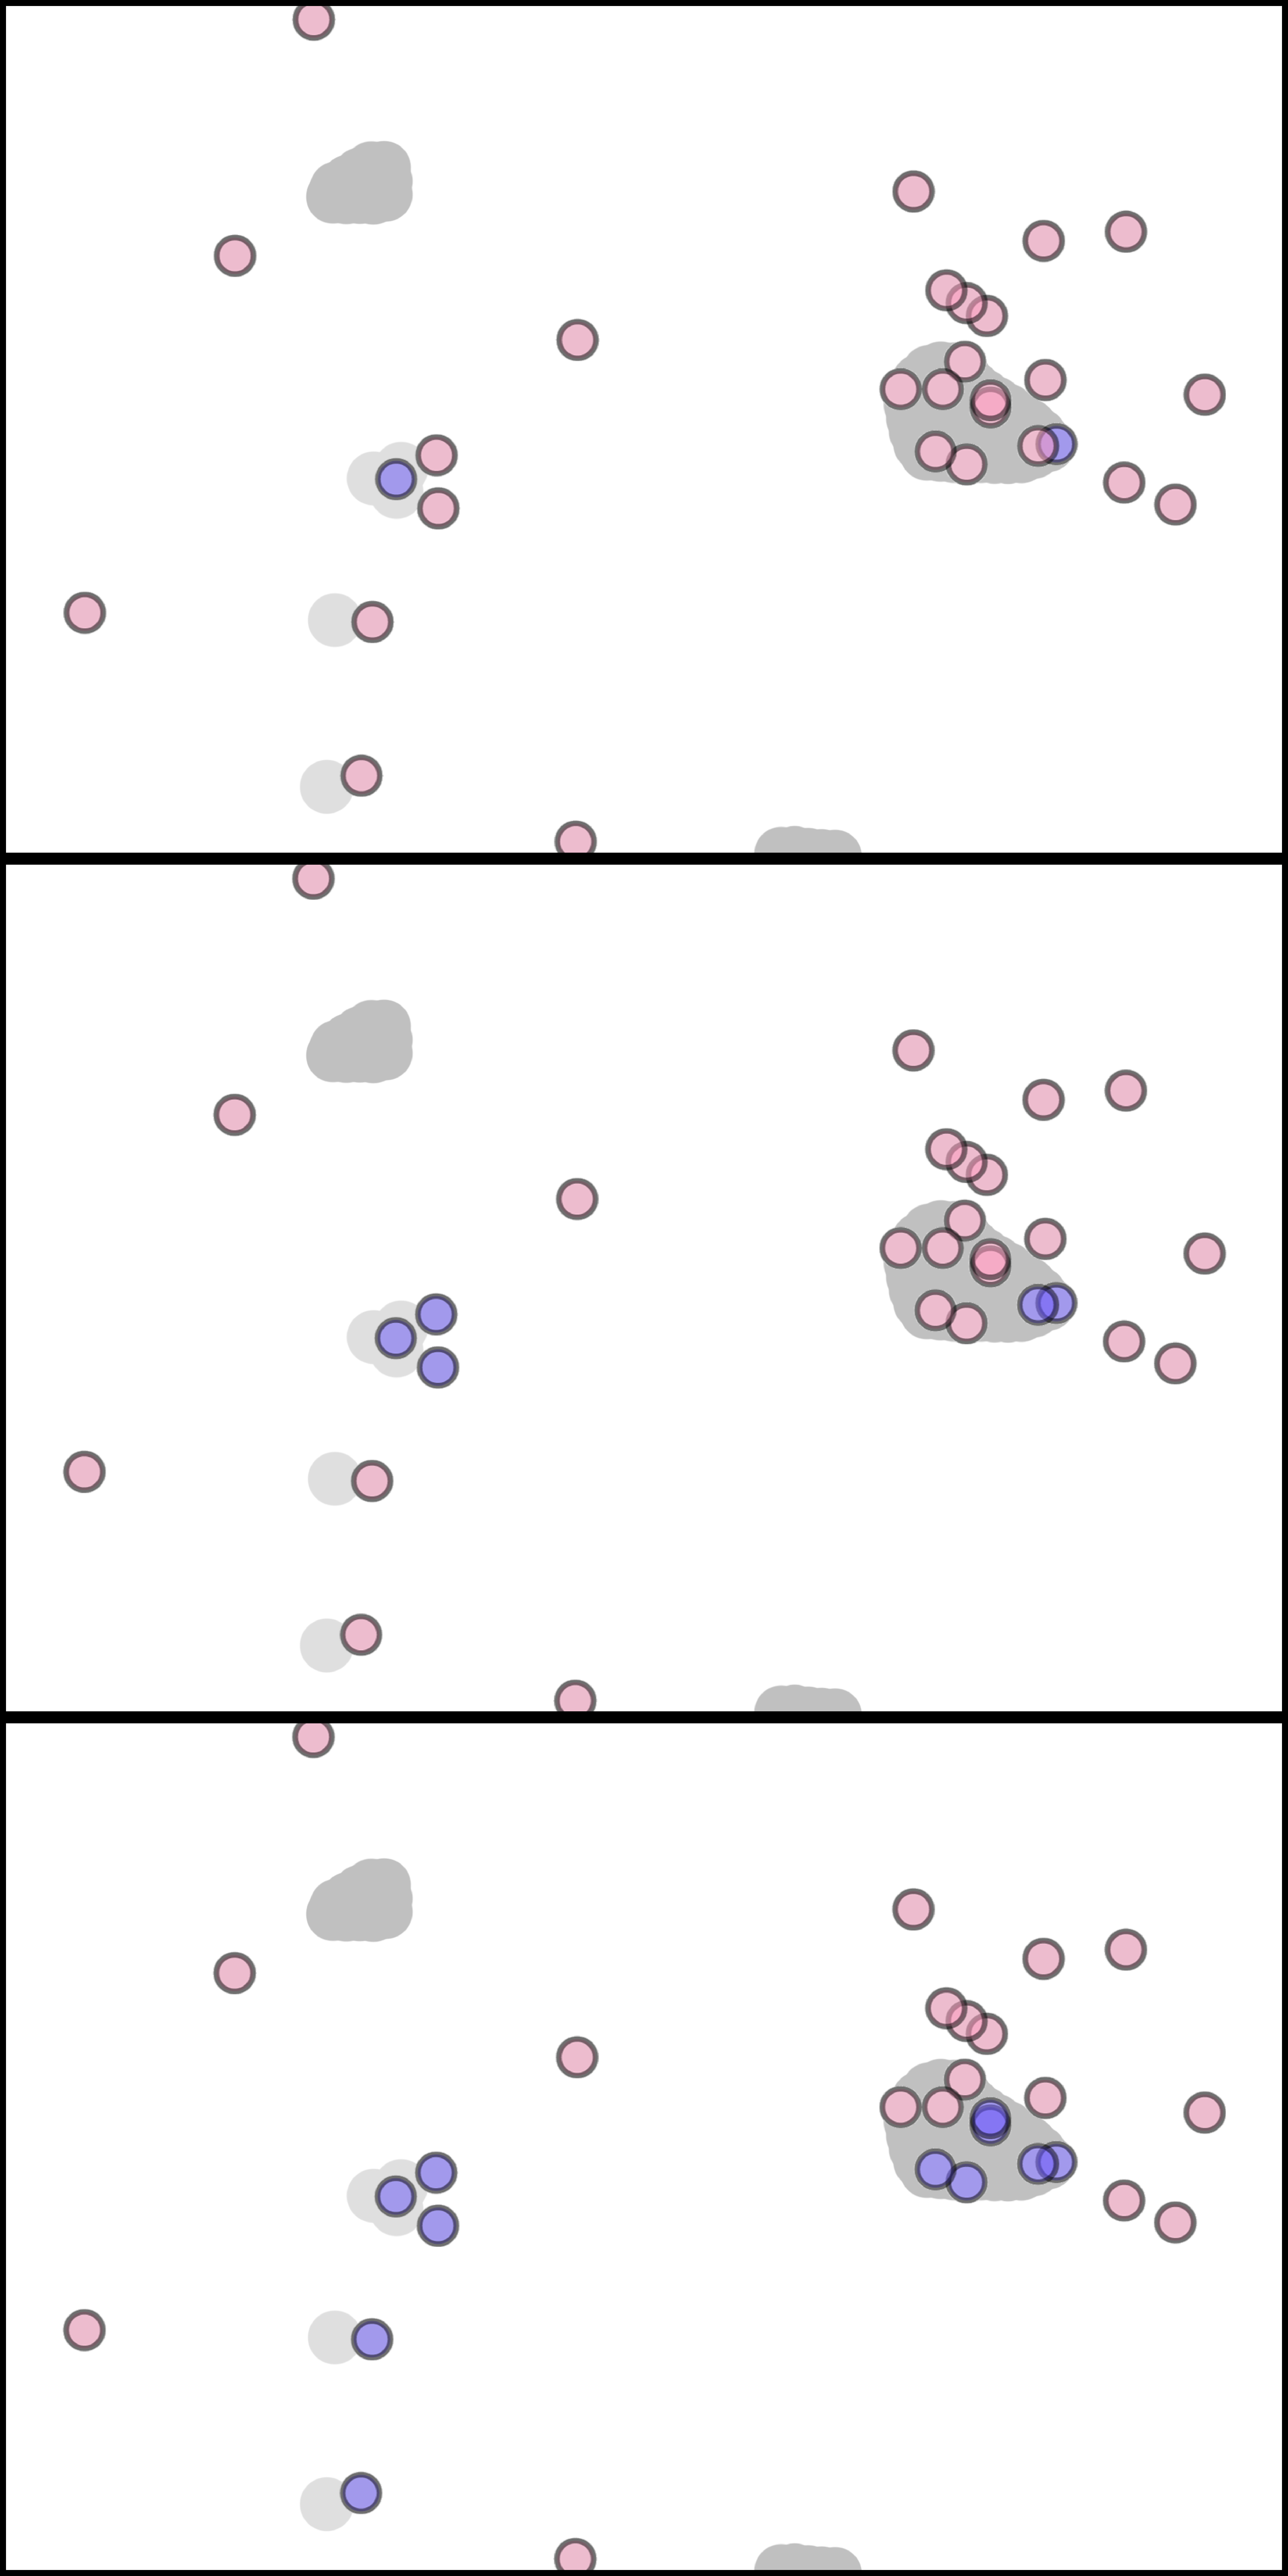
\includegraphics{figures/expansion-v} 

}

\caption{Example expansion over time from 2014 to 2016 (top to bottom) using fake data. Blue dots denote stores with Double Up, pink dots denote without. Gray sectors denote higher population density. The initial nodes can be seen in the top (2014) frame.}\label{fig:dufb-expansion}
\end{figure}

\hypertarget{methods}{\section{Methods}\label{methods}}

\chapter{Modeling of SNAP Consumption Cycle under MI benefits
schedule}\label{snap-consumption}

\begin{itemize}
\tightlist
\item
  Introduction
\item
  Data
\item
  Methods
\item
  Results
\item
  Conclusion
\end{itemize}

\bibliography{packages.bib,book.bib}


\end{document}
